% ============================================================================
% The Galactic Tidal-Radius Vignette: a worked example for NestyNet-SR
%
% This note accompanies the example directory examples/jacobi_tidal of the
% NestyNet-SR repository.  The text originated as a subsection of NestyNet
% Paper III and is distributed with the code so that the paper can cite the
% study compactly while the complete analysis remains available and
% reproducible alongside its data and results.
%
% Compile:  pdflatex jacobi_tidal_note.tex   (twice, for references)
% ============================================================================
\documentclass[11pt]{article}
\usepackage[margin=2.7cm]{geometry}
\usepackage{amsmath}
\usepackage{graphicx}
\usepackage[colorlinks=true,linkcolor=blue,citecolor=blue,urlcolor=blue]{hyperref}

\title{The Galactic Tidal-Radius Vignette:\\
Recovering the Jacobi Law and its Anisotropic Invariant\\
{\large A worked example distributed with NestyNet-SR}}
\author{Rodrigo A.\ Ibata, Wassim Tenachi, Foivos Diakogiannis,\\
Neil Ibata, Anirudh Shankar}
\date{August 2026}

\begin{document}
\maketitle

\begin{abstract}
\noindent
This note documents the galactic tidal-radius theory-discovery study
distributed with NestyNet-SR as \texttt{examples/jacobi\_tidal}.  From
mock star-cluster tables the pipeline discovers the anisotropic tidal
invariant $4\Omega^{2}-\kappa^{2}$ through its learned general-affine
determining operator and recovers the circular-orbit Jacobi radius law
in closed form, unifying the classical Hill/Roche and flat-rotation-curve
limits.  The study also measures the gradient-noise envelope of the
symmetry certificate and exhibits principled abstention at $1\%$
observational noise.  It serves as the controlled synthetic companion to
the SPARC baryonic-acceleration vignette of Paper~III
\citep{NestyNet2026b}.
\end{abstract}

\section{The problem}

As a theory-discovery case study with mock astronomical observables, we
ask the pipeline to recover the circular-orbit Jacobi (tidal) radius of a
star cluster or satellite in an axisymmetric galactic host,
%
\begin{equation}
r_J=\left(\frac{\mu}{4\Omega^{2}-\kappa^{2}}\right)^{1/3},
\qquad \mu = G M_{\rm cl},
\label{eq:jacobi-law}
\end{equation}
%
where $\Omega=v_c/R$ is the circular frequency and $\kappa$ the epicyclic
frequency of the cluster's orbit.  The tidal denominator
$q=(2\Omega)^{2}-\kappa^{2}$ is an \emph{anisotropic} indefinite quadratic
form, and two textbook approximations are its named limits.  For a
Keplerian rotation curve ($\kappa=\Omega$) it reduces to the Hill/Roche
radius $r_J=R\,(m/3M)^{1/3}$ (with $m$ the satellite mass and $M$ the
host mass enclosed within the orbital radius $R$), and for a flat
rotation curve ($\kappa^2=2\Omega^{2}$) to the classic
$r_J=R\,(m/2M)^{1/3}$ tidal radius (the King limit).  Discovering $q$
from data requires the generator
$V=\kappa\,\partial_\Omega+4\,\Omega\,\partial_\kappa$.  The isotropic
boost generator $\kappa\,\partial_\Omega+\Omega\,\partial_\kappa$ of the
fixed witness menu maps $q$ to $6\,\Omega\kappa$ rather than to zero, so
the vignette genuinely exercises the learned general-affine determining
operator of the generalized-symmetry layer \citep{NestyNet2026b} and not
a named detector.

\section{Table design and its two lessons}

Each table row is one cluster in its local tidal environment.  We draw
six host families with power-law rotation curves of logarithmic slope
$\alpha\in\{-\tfrac12,-\tfrac14,0,\tfrac14,\tfrac12,\tfrac34\}$
(spanning the Keplerian through rising-curve regimes), galactocentric
radii $R\in[2,50]$~kpc, cluster masses
$M_{\rm cl}\in10^{3.5\text{--}7}\,M_\odot$, and per-row scatter in the
local slope, with $\kappa^{2}=2(1+\alpha)\,\Omega^{2}$ and a $1\%$
lognormal observational error on $r_J$.  The regression inputs are
$(\mu,\Omega,\kappa)$ with dimension vectors $[\mu]=L^{3}T^{-2}$ and
$[\Omega]=[\kappa]=T^{-1}$, and no other information is supplied.

Two design facts matter and are themselves physically instructive.
First, a \emph{single} power-law host is uninformative.  On one host
$\kappa/\Omega$ is constant, every row lies on one ray of the
$(\Omega,\kappa)$ plane, and the determining operator correctly reports
a large degenerate symmetry algebra (including the isotropic boost)
rather than the tidal invariant.  The per-host alias
$r_J^{3}\propto\mu/\Omega^{2}$ fits perfectly.  At least two distinct
slopes pin the quadratic uniquely, and the slope scatter within hosts
gives the table two-dimensional support.  Second, that support controls
\emph{derivative} quality.  On a table confined to rays the surrogate
fits the function values to $10^{-4}$, but the gradient transverse to a
ray is then an extrapolation beyond the sampled locus and is in error by
$20\%$.  Filling the wedge between the rays samples that direction as
well and returns the transverse gradients to interpolation accuracy.

\section{Symmetry discovery and its noise envelope}

From the trained surrogate (values fitted to $3\times10^{-5}$, analytic
gradients accurate to $7\times10^{-5}$ relative), the affine determining
operator recovers the off-diagonal generator pair $(0.25,1.00)$ (that
is, $V=\kappa\,\partial_\Omega+4\,\Omega\,\partial_\kappa$) at
confidence $0.991$, giving the discovered invariant
%
\begin{equation}
\hat q = 4.027\,\Omega^{2}-\kappa^{2},
\end{equation}
%
whose correlation with the observed tidal curvature $\mu/r_J^{3}$ is
$0.999999$ over more than four decades of tidal curvature.  As a
by-product the same operator discovers that the tidal curvature is
homogeneous of degree $2.000$ in the frequencies (Euler output action
$\beta=2$).  The gradient-quality envelope is sharp and was measured
directly by perturbing exact gradients.  The invariant is accepted up
to relative gradient errors of ${\sim}10^{-3}$, still correctly
classified at $3\times10^{-3}$, and lost by $10^{-2}$.  At the $1\%$
observational noise of the fiducial table, capacity-controlled
surrogate gradients plateau at $1.3\times10^{-2}$, and the one-shot
operator then declines to certify any invariant and does not produce a
false one.  Only the (along-ray) homogeneity survives, essentially
unimpaired.  Symmetry discovery from a fitted surrogate thus inherits
the surrogate's derivative quality, the central theme of Paper~I
\citep{NestyNet2026a}, and precise data, or curvature-supervised
surrogate training, is what buys the full invariant.

\section{End-to-end closed-form recovery}

The end-to-end pipeline, run with units enabled, with the
generalized-symmetry Stage-A layer active, and with $6\,000$ training
and $2\,000$ validation rows, completes the recovery in closed form.
On precise data, Stage~A autonomously factors the law along its
homogeneity structure, $r_J = f(\mu)\cdot F(\Omega/\kappa)\cdot
g(\Omega)$, discovering the dimensionless ratio $\Omega/\kappa$ as an
internal coordinate.  Stage~B then closes the mass factor as a
free-exponent power law with exponent $0.3333332$ (the cube root of
Eq.~\eqref{eq:jacobi-law}, recovered to five parts in $10^{7}$) and
closes the dimensionless profile exactly as $(4-t^{2})^{-1/3}$, the
cube root of a polynomial in the discovered ratio.  The fitted
quadratic is $4.000\,\Omega^{2}-\kappa^{2}$ to machine precision (the
linear coefficient is driven below $10^{-15}$ and pruned), reached at
validation loss $8\times10^{-33}$ with three parameters, so the
assembled expression is Eq.~\eqref{eq:jacobi-law} itself, with no
residual neural factor.

Reaching it depends on the two design facts made explicit above.  The
wedge-filling ensemble supplies the two-dimensional support without
which a reciprocal-cubic or rational approximant is numerically
indistinguishable from the exact cube root on any single
ratio-restricted subsample, and the closure library must contain a
cube-root-of-polynomial map alongside its square-root and reciprocal
siblings.  With both present, the search rejects several hundred
plausible-but-wrong closed forms against a $2.7\times10^{-10}$ neural
baseline, including the rational approximants that are only good enough
on a restricted subsample, and selects the exact cube root, which is
simultaneously the most accurate closure and, at three parameters, the
parsimony winner.  On the $1\%$-noise table the same pipeline keeps the
neural fit and proposes no closure at all.  The noise-limited surrogate
cannot be certified below the acceptability gate (validation loss
$5.9\times10^{-6}$ against a $4.1\times10^{-6}$ threshold), so the
search declines to enter the closure stage rather than fit a spurious
analytic form to noise.  Its nearest structural attempt is instructive,
the compound-variable detector reaching for a single tidal factor
$z=2\Omega-\kappa$, one root of
$4\Omega^{2}-\kappa^{2}=(2\Omega-\kappa)(2\Omega+\kappa)$, which it
rejects because a lone linear factor leaves a systematic residual.  As
with the symmetry layer, the closure inherits the surrogate's
precision.  The exact law is recovered on precise data, while noise is
met with abstention rather than a false positive.

\begin{figure}[t]
\centering
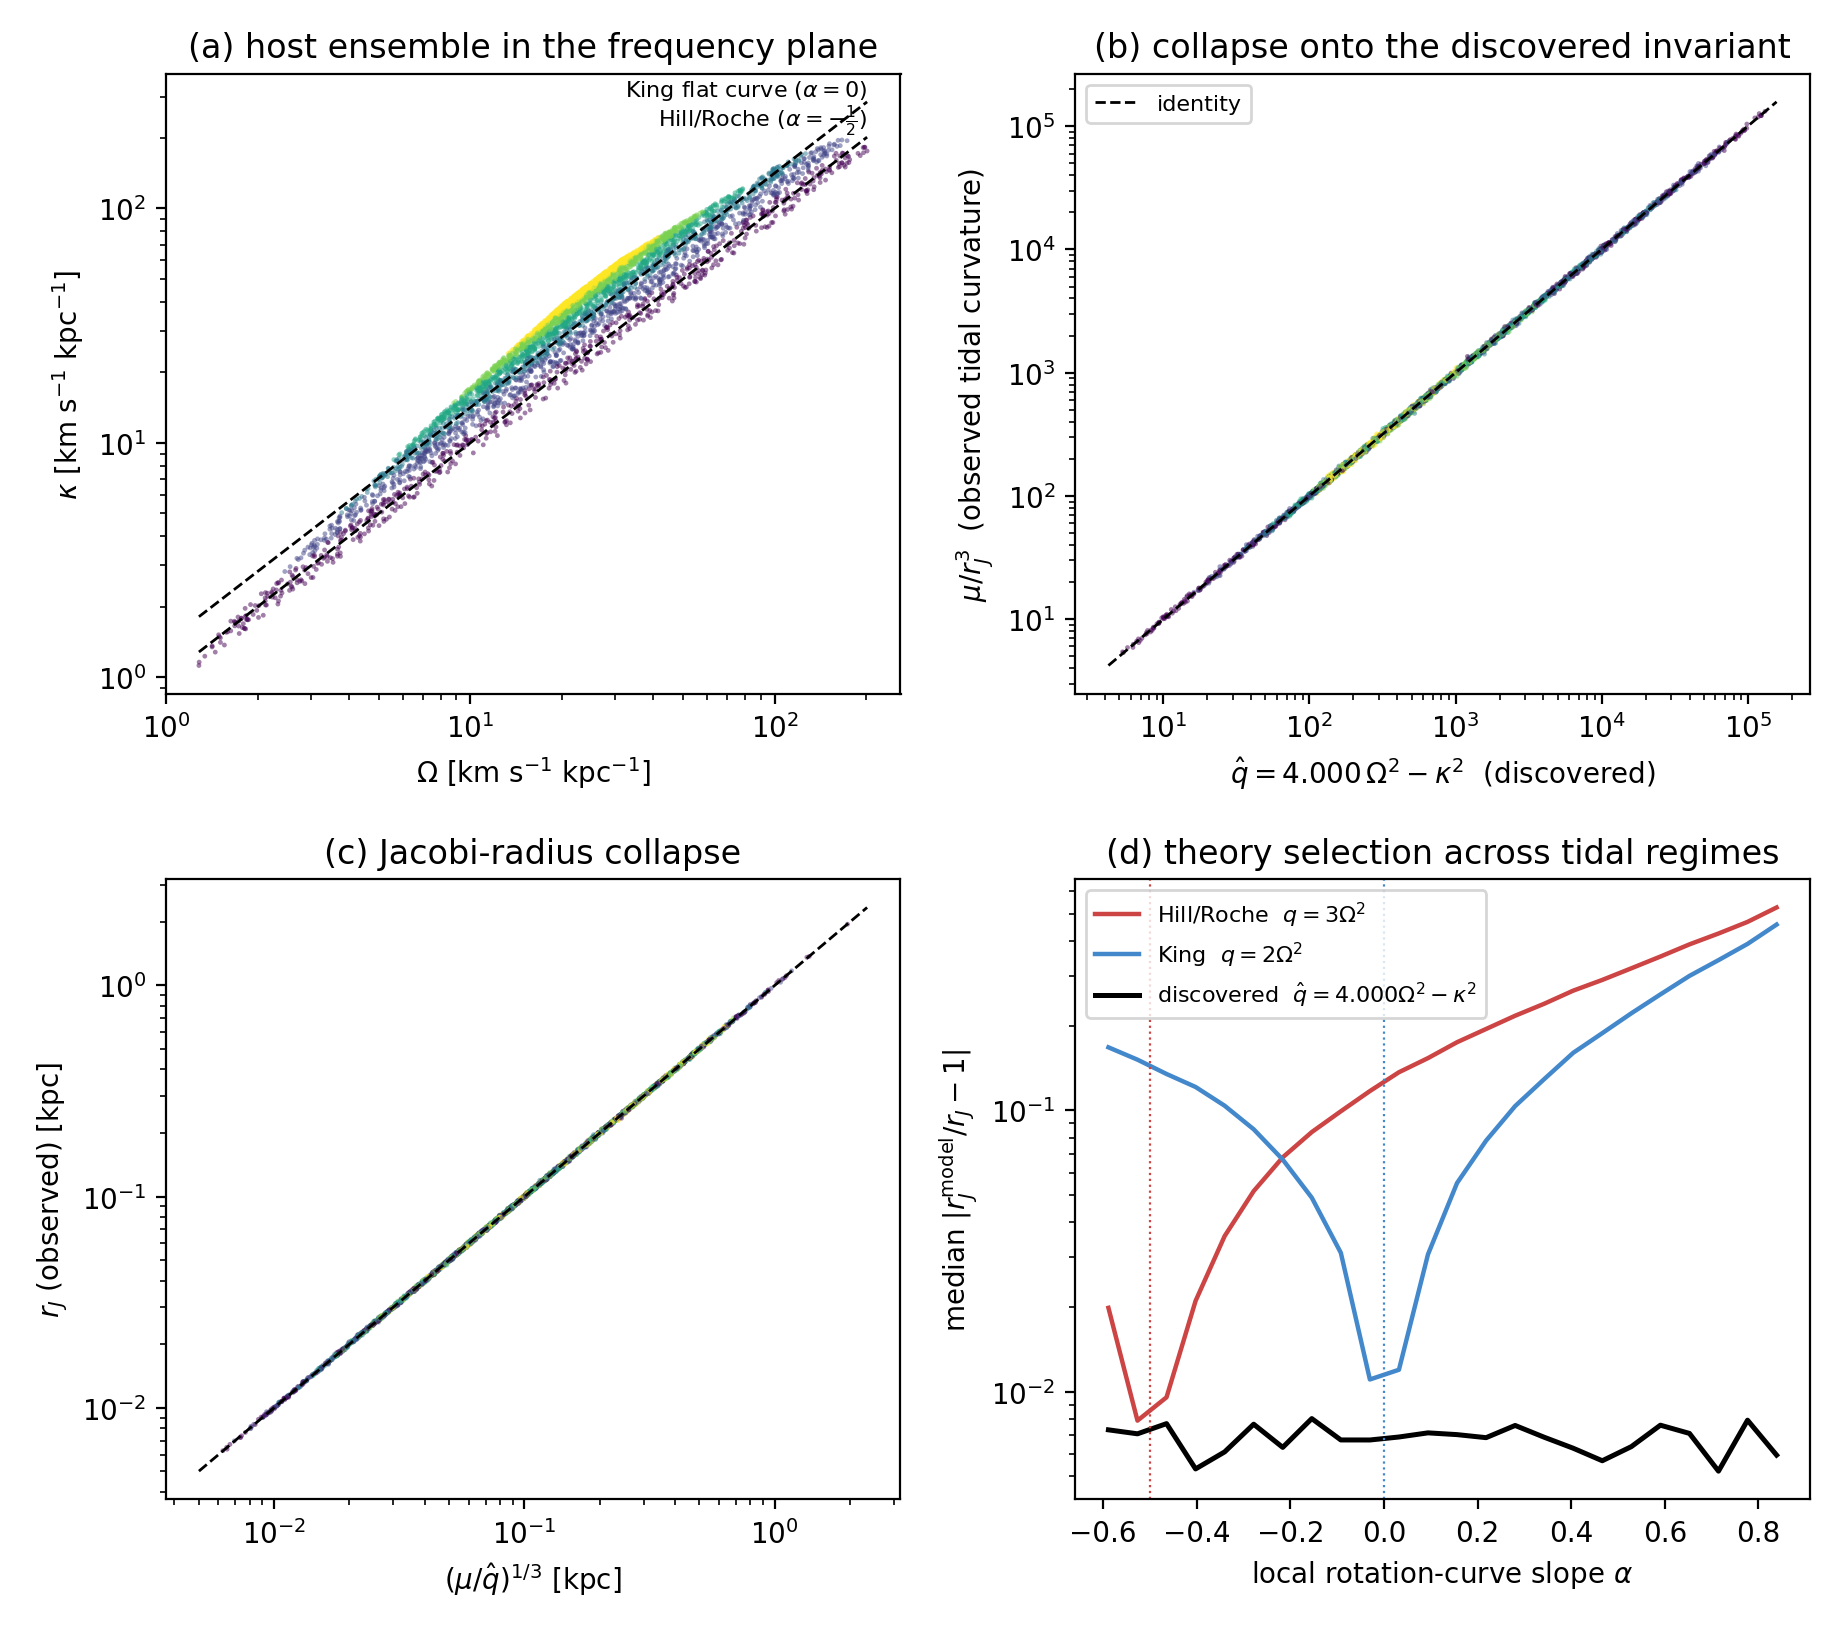
\includegraphics[width=\textwidth]{figures/jacobi_vignette_quadpanel.png}
\caption{The tidal-radius vignette.  (a)~The six-host ensemble in the
$(\Omega,\kappa)$ plane.  The dashed rays are the Keplerian
(Hill/Roche) and flat-curve (King) limits, and the per-row slope
scatter fills the wedge between host families.  (b)~Collapse of the
observed tidal curvature $\mu/r_J^{3}$ onto the discovered invariant
$\hat q=4.000\,\Omega^{2}-\kappa^{2}$, over more than four decades.
(c)~The assembled Jacobi-radius law against the observations.
(d)~Theory selection across tidal regimes.  The Hill/Roche and
flat-curve approximations are exact only at their home slopes
($\alpha=-\tfrac12$ and $\alpha=0$, dotted lines), while the discovered
law, having recovered the invariant exactly, sits flat below $1\%$, at
the observational noise floor, across the full range.}
\label{fig:quadpanel}
\end{figure}

Figure~\ref{fig:quadpanel} summarizes the vignette.  Panel~(d) is the
theory-level payoff.  The two classic approximations fail away from
their home regimes exactly as they should, while the single discovered
law (one invariant, one cube root) explains every tidal environment at
the observational floor.  The vignette thus exhibits the intended
division of labor.  The generalized-symmetry layer discovers the
anisotropic carrier that no fixed library contains, the separability
machinery factors the law along the symmetry's homogeneity structure,
and the closure rules recover both the rational exponents and the
cube-root profile in closed form.

\section{Reproduction}

The example directory contains the cluster tables
(\texttt{data/jacobi\_master.csv} and the derived
\texttt{jacobi\_v1\_full.csv}, \texttt{jacobi\_v2\_cube.csv},
\texttt{jacobi\_v3\_carrier.csv}, with provenance in
\texttt{data/jacobi\_manifest.json}), the run logs and reports under
\texttt{results/}, and this figure under \texttt{figures/}.  The
end-to-end invocation is recorded in
\texttt{results/reroll\_harness.log} and follows the fixed benchmark
configuration of Paper~III with the generalized-symmetry flags enabled:
%
\begin{verbatim}
python3 -u -m nestynet_sr.run_SR \
  --filepath examples/jacobi_tidal/data/jacobi_v1_full.csv \
  --units_basis "L,T,M" --y_units "[1,0,0]" \
  --x_units "[[3,-2,0],[0,-1,0],[0,-1,0]]" \
  --gs-stagea --gs-general-affine --gs-noise-calibrated-promotion \
  --ndata_train 6000 --ndata_val 2000
\end{verbatim}

\begin{thebibliography}{2}
\bibitem[Ibata et al.(2026a)]{NestyNet2026a}
Ibata, R.~A., Tenachi, W., Diakogiannis, F., Ibata, N., \& Shankar, A.\
2026a, NestyNet.\ I.\ Physics Functions Are Hard to Fit with Neural
Networks: A Framework for Accurate Surrogates and Analytic Derivatives,
ApJ, in preparation

\bibitem[Ibata et al.(2026b)]{NestyNet2026b}
Ibata, R.~A., Tenachi, W., Diakogiannis, F., Ibata, N., \& Shankar, A.\
2026b, NestyNet.\ III.\ Symbolic Regression from Analytic Neural
Surrogates, ApJ, in preparation
\end{thebibliography}

\end{document}
